\documentclass{article}
\usepackage{arxiv}

\usepackage[utf8]{inputenc} % allow utf-8 input
\usepackage[T1]{fontenc}    % use 8-bit T1 fonts
\usepackage{hyperref}       % hyperlinks
\usepackage{url}            % simple URL typesetting
\usepackage{booktabs}       % professional-quality tables
\usepackage{amsfonts,amssymb,amsmath}       % blackboard math symbols
\usepackage{nicefrac}       % compact symbols for 1/2, etc.
\usepackage{microtype}      % microtypography
\usepackage{lipsum}
\usepackage{graphicx}
\usepackage{float}
\graphicspath{ {./images/} }


\title{Crypto Momentum Portfolios}


\author{
 Jules Prieux \\
  Paris-Dauphine University\\
  Paris, 75016  \\
  \texttt{jules.prieux@dauphine.eu} \\
  %% examples of more authors
   \And
 Ahmed Bachir \\
  Paris-Dauphine University\\
  Paris, 75016 \\
  \texttt{ahmed.bachir@dauphine.eu} \\
  \And
 Baptiste Zloch \\
  Paris-Dauphine University\\
  Paris, 75016 \\
  \texttt{baptiste.zloch@dauphine.eu} \\
  %% \AND
  %% Coauthor \\
  %% Affiliation \\
  %% Address \\
  %% \texttt{email} \\
  %% \And
  %% Coauthor \\
  %% Affiliation \\
  %% Address \\
  %% \texttt{email} \\
  %% \And
  %% Coauthor \\
  %% Affiliation \\
  %% Address \\
  %% \texttt{email} \\
}

\begin{document}
\maketitle
\begin{abstract}

	In the ever-evolving landscape of cryptocurrency investment, this research paper draws inspiration from financial luminaries Titman et al. (1993) \cite{Titman1993} and Moskowitz et al. (2011) \cite{Moskowitz2011} to craft a sophisticated approach tailored to the unique characteristics of Bitcoin (BTC). \newline
	Our study undertakes a comprehensive exploration of the dataset's statistical properties and crafts bespoke momentum signals for cryptocurrency markets. Leveraging these signals, we design a cutting-edge quantitative investment strategy encompassing market timing for both long and short positions, along with long-short and long-only frameworks using a cross-sectional approach. We meticulously analyze historical price data to extract meaningful insights into the statistical nuances of the cryptocurrency market, fashioning robust momentum signals that align with the idiosyncrasies of digital assets. Our strategies empower active market participation, enabling investors to seize short-term trends in BTC performance. Through rigorous backtesting, we evaluate and compare strategy performance against a market cap-weighted benchmark.This research not only advances cryptocurrency investment strategies but also contributes to the broader discourse on applying traditional financial models to digital assets. By distilling our findings, we offer nuanced perspectives for academics and practitioners navigating the dynamic world of cryptocurrency investments.
\end{abstract}



\keywords{Cryptocurrencies \and Asset pricing \and Time series \and Portfolio management}
\section{Introduction}\label{sec:introduction}
\section{Data}\label{sec:data}
Jules
\section{Methodology}
\subsection{Notations}
In the following pages we present the methodology to run a momentum strategy against a benchmark. We use different notations
\begin{itemize}
	\item $X$ is the distribution of the return it could be parametric or non-parametric
	\item $p_i$ is a scalar representing the i-th daily price
	\item $r_{p_i}$ is the scalar representing the i-th daily return.
	\item $r_p$ is a vector representing all the returns of the portfolio
	\item $r_b$ is a vector representing all the returns of the benchmark
	\item $r_F$ is the scalar representing the risk-free rate
	\item $\sigma_i^k$ is a scalar representing the volatility on a window $k$ at time point $i$
	\item $w_k$ is a scalar representing the weight for an asset $k$
	\item $w_{k,i}$ is a scalar representing the weight of the asset $k$ at time $i$
	\item $r_{k,i}$ is a scalar representing the return of the asset $k$ at time $i$
	\item $w$ is a vector representing the weight of $n$ assets.
\end{itemize}

\subsection{Benchmarks definition}
We aim to conduct multiple backtests to assess the viability of momentum factor investing in cryptocurrencies. To evaluate the performance of the momentum strategy, it is imperative to establish baseline benchmarks. Accordingly, we will delineate three distinct benchmarks:
\begin{itemize}
	\item \textbf{A market capitalization weighted benchmark}: This benchmark encompasses the entire spectrum of cryptocurrencies, with weights allocated proportionally to the market capitalization of each asset.
	\item \textbf{An equally weighted benchmark}: This benchmark includes the entire array of cryptocurrencies, with each asset assigned an identical weight.
	\item \textbf{BTC-USDT benchmark}: Here, Bitcoin is employed as the benchmark due to its widespread recognition and status as the most extensively traded cryptocurrency.
\end{itemize}

\begin{figure}[H] % picture
	\centering
	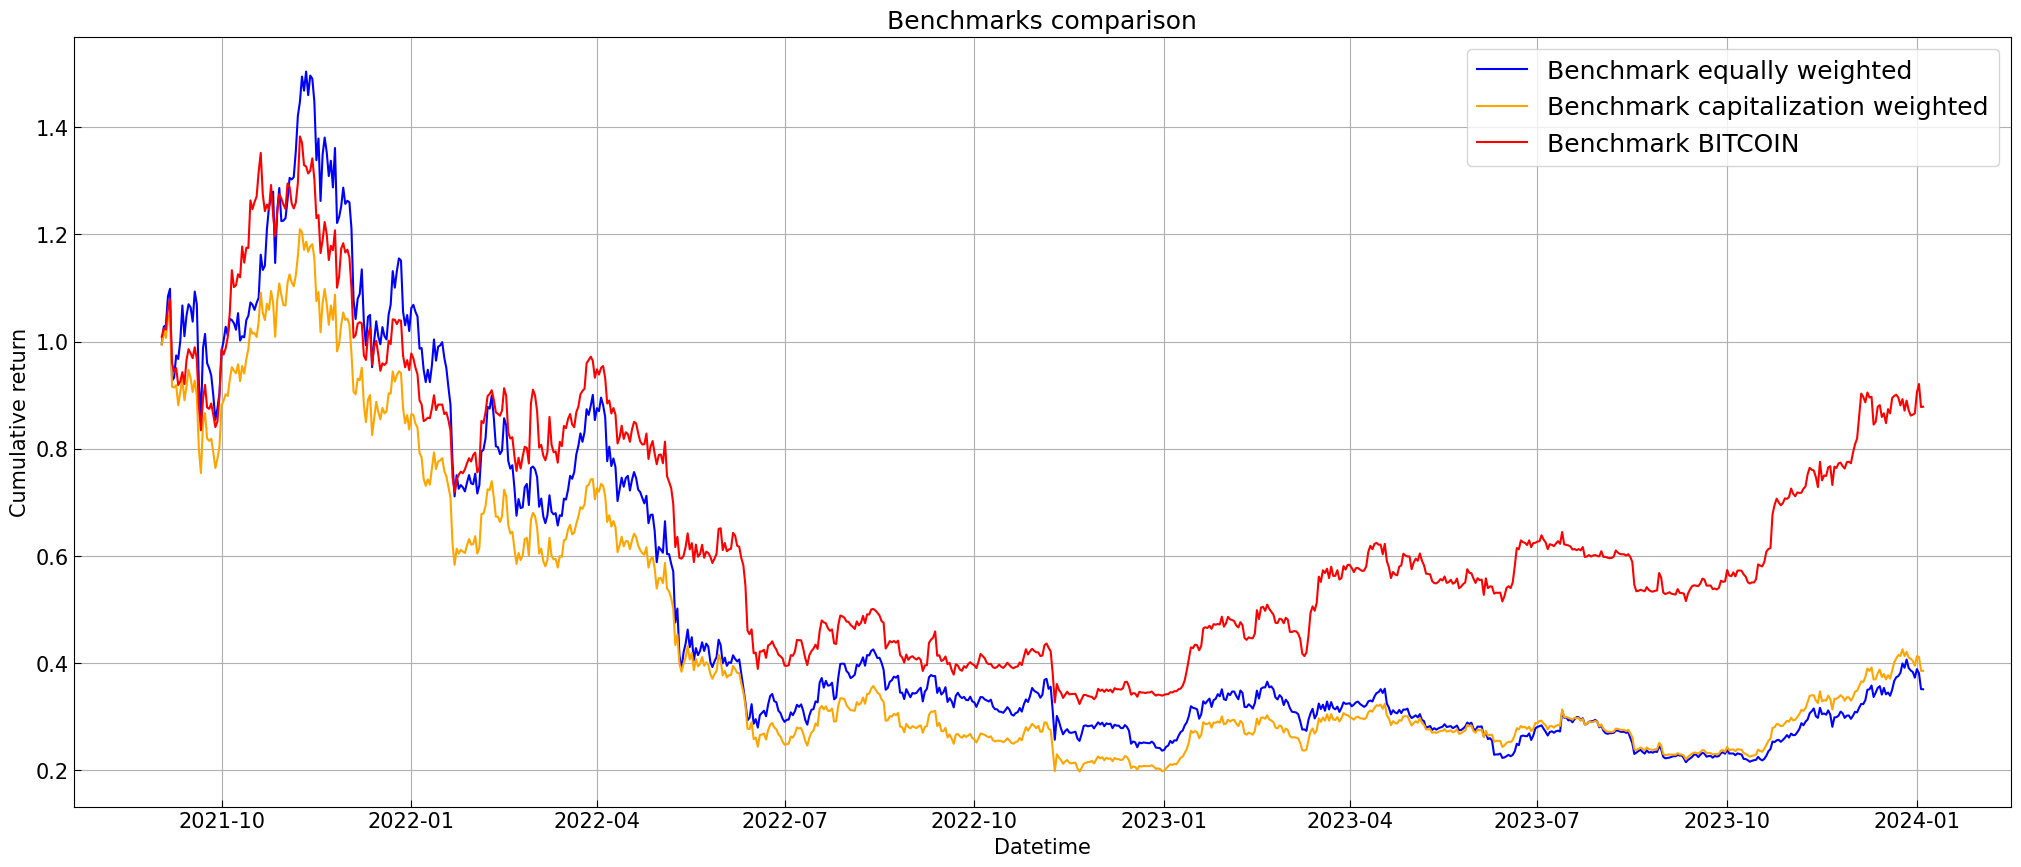
\includegraphics[width=1\linewidth]{benchmarks_only.png}
	\caption{The historical track of the 3 benchmarks used in this paper}
	\label{fig:fig1}
\end{figure}

\subsection{Performance and risk metrics}
To gauge the effectiveness of various iterations of the momentum strategy, we will employ the following set of performance metrics and risk metrics. All the metrics computed will be presented as annualized in the section \ref{sec:mainres}.


The \textbf{expected return} (\(r_P\)) is a scalar denoting the average gain or loss an investor can anticipate. It is computed as the arithmetic mean of individual returns:
\[r_P=\mathbb{E}[r_p]=\Bar{r_p}=\frac{1}{N}\sum_{i=1}^Nr_{p_i}\]

The historical \textbf{volatility} (\(\sigma_P\)) serves as a risk measure, representing the standard deviation of returns around the mean over a specific period:
\[\sigma_P = \sqrt{\frac{1}{N-1}\times\sum^N_{i=1}(r_{p_i}-\Bar{r_p})^2}\]

The historical \textbf{value-at-risk (VaR)} is a risk measure denoting the potential loss at a specified percentile of the returns distribution (\(1-\alpha\)):
\[\text{VaR}_{1-\alpha}(X)=\text{inf}_{t\in\mathbb{R}}\{t:P(X\leq t)\geq1-\alpha\}\]

The historical \textbf{conditional value-at-risk (CVaR)} is the average loss for extreme returns, usually conditioned as lower than the value-at-risk:
\[\text{CVaR}_{1-\alpha}(X)=\frac{1}{\alpha}\int_\alpha^\beta\text{VaR}_{1-\gamma}(X)d\gamma\]

The \textbf{beta} (\(\beta\)) represents the sensitivity of a strategy to a benchmark. A beta greater than 1 implies an overreaction to benchmark changes:
\[\beta = \frac{\text{cov}(r_p,r_b)}{\sigma_B^2}\]

The \textbf{tracking error} (\(\text{TE}\)) measures the average deviation of the strategy from a benchmark, providing an ex-post risk measure:
\[\text{TE}=\sqrt{\mathbb{V}(r_p-r_b)}\]

The \textbf{Sharpe ratio} (\(\text{SR}\)) is an absolute performance measure, quantifying the excess return from a strategy per unit of volatility:
\[\text{SR} = \frac{r_P-r_F}{\sigma_P}\]

The \textbf{information ratio} (\(\text{IR}\)) is a relative performance measure for portfolio management, replacing the risk-free rate with the benchmark expected return and using tracking error in the denominator:
\[\text{IR} = \frac{r_P-r_B}{TE}\]

The \textbf{tail ratio} (\(\text{TR}\)) is a risk measure, representing the ratio of conditional average gain over the inverse conditional loss. A value greater than one indicates an asymmetric strategy with positive extreme returns higher than negative extreme returns:
\[\text{TR}=\frac{\text{CVaR}_{0.05}(X)}{\text{CVaR}_{0.95}(X)}\]


All these metrics will be detailed in section\ref{sec:mainres}, accompanied by their respective t-statistics. The inclusion of t-statistics is crucial for evaluating the significance of the strategy in comparison to the benchmark. Considering the limited historical data comprising approximately 700 data points, we opted for a statistical bootstrap sampling with replacement approach. This technique involves the random selection of 200 returns from the available 700 data points, repeated 1000 times. With each iteration, we compute the entire suite of metrics, allowing us to conduct a two sided t-test. The hypotheses for the t-test are as follow:
\begin{itemize}
	\item $H_0$ : The strategy computed metric is the equal to the benchmark computed metric
	\item $H_1$ : The strategy computed metric is different from the benchmark computed metric
\end{itemize}

\subsection{Different momentum formula}\label{sec:momentumformulas}
Momentum in finance denotes the tendency of assets that have demonstrated robust performance, either positively or negatively, in the past, to persist in their price movements in the same direction for a specific period Titman et al. (1993)\cite{Titman1993}. The fundamental premise of momentum investing is grounded in the belief that assets that have recently performed well are likely to continue performing positively, while those that have performed poorly are likely to persist in underperformance Asness et al. (2009)\cite{Asness2009}.
\newline
In practical terms, there exist various methods for quantifying the best and worst performers over a given period. Consequently, this paper aims to distinctly define four approaches for calculating asset momentum to facilitate the backtesting of these different momentum strategies.
\newline
The four distinct momentum formulas are articulated as follows:
\newline\newline
\textbf{Price momentum} : given an asset prices time series $\{p_1, p_2, ..., p_n\}$ at each point $i$ the $k$-periods price momentum is computed as : $$\textit{price momentum}^{k}_i = \frac{p_i}{p_{i-k}}$$ \newline

\textbf{Time series momentum} : This formula is directly applied from Moskowitz et al. (2011) \cite{Moskowitz2011}. Given a time series of daily returns $\{r_1, r_2, ..., r_n\}$ and its associated $k$-periods rolling volatility $\{\sigma_1^k, \sigma_2^k, ..., \sigma_n^k\}$ then at each point $i$, the 1 year TSMOM is computed as follow: $$\textit{TSMOM}^{365}_{i}=\text{sign}(r_{i-12})\times\frac{40\text{\%}}{\sigma_i^365}\times r_i$$ \newline
\textbf{Moving average momentum} : The moving average momentum is basically the potential return of the price over the its exponential moving average. A high and positive distance indicates a strong momentum. Therefore given an asset prices time series $\{p_1, p_2, ..., p_n\}$ then we compute the exponential moving average over $k$ periods with the following formula : $\textit{EMA}^k_i=\frac{1}{k}\sum_{j=0}^k \alpha\times(1-\alpha)^j\times p_i-j$. Now their is  another time series $\{\text{EMA}_1^k, \text{EMA}_2^k, ..., \text{EMA}_n^k\}$. Then the moving average momentum at each point $i$ is computed as follow: $$\textit{EMAMOM}^k_i=\frac{p_i}{EMA_i^k}$$\newline

\textbf{Volatility-neutralized momentum} : The concept of volatility-neutralized momentum aligns with price momentum, albeit with an additional consideration for mitigating the impact of noise inherent in price movements. This is achieved by normalizing the volatility effect, wherein the price momentum is divided by the volatility over the same period during which the price momentum is computed. Given a time series of daily returns $\{r_1, r_2, ..., r_n\}$ and its associated $k$-periods rolling volatility $\{\sigma_1^k, \sigma_2^k, ..., \sigma_n^k\}$ then at each point $i$, the volatility-neutralized momentum formula is articulated as follows: $$\textit{vol neutral momentum}^{k}_i = \frac{p_i}{p_{i-k}}\times\frac{1}{\sigma_i^k}$$
Remark : Only the TSMOM is can be negative therefore we will not use it to perform asset allocation.
\subsection{Backtest implementation}
Backtesting a strategy is a quantitative methodology used to assess the historical performance of an investment strategy based on past market data. In essence, it involves applying a set of predefined rules or algorithms to historical market data to simulate how the strategy would have performed over a specific time period. The primary goals of backtesting are to evaluate the strategy's effectiveness, understand its historical risk and return characteristics, and gain insights into its potential future performance. Therefore to be relevant backtest must assert that a each iteration the future data points are unknown it has to be an online process.
\newline
In order to backtest an investment strategy we have to define several things. First of all we need to provide a universe. The universe is described in the section \ref{sec:data} and \ref{sec:descstats}. Then we need to specify the asset selection method and asset allocation method. Theses methods represent the strategy's decisions made over time at each rebalance period. At each rebalance date, all the previous securities in the portfolio are sold. Then the new cash is available and ready to be invested in the newly selected securities.

\subsubsection{Asset selection}
To implement the strategy we need to define the asset selection methodology. As we focus on momentum based investment in this research paper, the asset selection will be performed by ranking in descending order the universe's securities by their momentum. The word momentum here refers to the formulas defined in the section \ref{sec:momentumformulas}. Once the securities are sorted the algorithm select the $k$ best performing cryptocurrencies. $k$ here is a user defined input, also know as hyperparameter of the strategy, like the momentum window, etc.
\subsubsection{Asset allocation}
As the asset selection has been performed, the next step is to allocate a fraction of the cash in the newly selected assets. In this paper we would also like to find the best way to allocate the assets given a momentum calculation. Therefore we used five different asset allocate methods:\newline\newline
\textbf{Equally weighted allocation} : The equally weighted allocation is the most simple one, the fraction of cash invested in each securities is the same. Therefore the weight for the asset $i$ given $n$ assets in the portfolio is the following: $$w_k=\frac{1}{n}$$
\textbf{Capitalization weighted allocation} : The capitalization weighted allocation is quite simple the fraction of cash invested in each securities is proportional to the market capitalization of each asset selected. Therefore the weight for the asset $i$ given $n$ assets in the portfolio is the following: $$w_k=\frac{\textit{market cap}_k}{\sum_{j=0}^n\textit{market cap}_j}$$
\textbf{Momentum weighted allocation} : momentum weighted allocation is quite simple the fraction of cash invested in each securities is proportional to the momentum of each asset selected. Therefore the weight for the asset $i$ given $n$ assets in the portfolio is the following: $$w_k=\frac{\textit{momentum}_k}{\sum_{j=0}^n\textit{momentum}_j}$$
\textbf{Mean variance allocation} : The mean variance allocation is a bit more complex than the three previous one. This one in basically a convex optimization problem. Our output is a line vector containing the weight for each asset, this is the vector $w$. Then we need to define the objective function: $$f(w)=\frac{\mathbb{E}[r_P]}{\sigma_P}$$
where:
\begin{itemize}
	\item $\sigma_P=\sqrt{w^T \Sigma w}$ is the volatility of the portfolio
	\item $\mathbb{E}[r_P]=w \cdot R$ is the expected return of the portfolio
	\item $\Sigma$ is the variance-covariance matrix of the $n$ assets returns
	\item $R$ a column vector containing the expected returns for each of the $n$ assets.
\end{itemize}
The optimization problem is to find the weights $w$ that maximize the objective function subject to constraints:
\[
	\begin{cases}
		\textbf{} & w^*=\text{argmax}(f(w))                                                    \\
		\text{}   & \text{s.t.} \quad\sum_{i=1}^{n} w_i = 1 \quad \text{(sum of weights is 1)} \\
		\text{}   & \text{s.t.} \quad w_i \geq 0 \quad \text{(long-only portfolio)}
	\end{cases}
\]
\newline
\textbf{Risk parity allocation} : The risk parity allocation Roncalli et al. (2008)\cite{Maillard2008} is a even more complex than the previous one. This one in basically a convex optimization problem. But in this case the aim is to allocate equally the risk contribution of the $n$ asset in the portfolio. A very risky asset will have a lower weight. Our output is a line vector containing the weight for each asset, this is the vector $w$. Then we define the objective function, this is defined as the squared Euclidean norm of the difference between actual risk contributions (\(AC\)) and target risk contributions (\(TRC\)):

$$f(w) = \lVert AC - TRC \rVert^2=\left\lVert \begin{bmatrix} RC_1 \\ RC_2 \\ \vdots \\ RC_n \end{bmatrix} - \begin{bmatrix} \frac{1}{n} \sigma_P \\ \frac{1}{n} \sigma_P \\ \vdots \\ \frac{1}{n} \sigma_P \end{bmatrix} \right\rVert^2$$

where:
\begin{itemize}
	\item $RC_k = \frac{\partial \sigma_P}{\partial w_k}$ is the risk contribution of each asset
	\item $\sigma_P=\sqrt{w^T \Sigma w}$ is the volatility of the portfolio
	\item $\Sigma$ is the variance-covariance matrix of the $n$ assets returns
\end{itemize}

The optimization problem is to find the weights $w$ that maximize the objective function subject to constraints:

\[
	\begin{cases}
		\text{} & w^*=\text{argmax}\{\lVert AC - TRC \rVert^2\}                              \\
		\text{} & \text{s.t.}\quad \sum_{i=1}^{n} w_i = 1 \quad \text{(sum of weights is 1)} \\
		\text{} & \text{s.t.}\quad w_i \geq 0 \quad \text{(long-only portfolio)}
	\end{cases}
\]

Allocation adjustments are executed at each rebalance date, occurring at periodic intervals such as weekly, monthly, or quarterly occurrences. Notably, the backtesting procedure must consider the phenomenon of weight drift. As the portfolio's assets evolve on a daily basis, ensuring that the sum of weights remains constant at 1, the weights undergo daily adjustments. The weight drift is mathematically expressed by the following formula:

$$w_{k,i}=\frac{w_{k,i-1} (1+r_{k,i})}{\sum_{j=1}^n w_{j,i-1}(1+r_{j,i})}$$

In each iteration of the backtest implementation, the following formula is employed to enhance the realism of the simulation.
\subsubsection{Transaction costs and slippage effect}
To enhance the realism of our backtesting process, we incorporate transaction costs at each rebalance date, reflecting the expenses incurred in selling all existing securities and acquiring new ones. Given that our asset universe comprises cryptocurrencies, we implement transaction costs based on those observed on the Binance exchange, a prominent platform in this domain. Specifically, for both buying and selling a security, a transaction cost of 0.1\% of the nominal value is applied. Market orders are exclusively utilized, thereby incurring taker fees.\newline\newline
Additionally, the execution of market orders exposes us to the slippage effect, denoting the marginal difference between the intended transaction price and the actual executed price. Such disparities may arise due to bid-ask spreads or liquidity constraints. We posit that the slippage effect consistently amounts to 0.05\% per transaction.

\section{Descriptive statistics}\label{sec:descstats}
Ahmed
\section{Main results}\label{sec:mainres}
\subsection{Optimal momentum and re-balance period}
Jules
\subsection{Optimal momentum calculation}
Ahmed
\section{Robustness}\label{sec:robustness}
Jules
\section{Conclusion}
\section{Appendix}
\bibliography{references}
\bibliographystyle{unsrt}
\end{document}
%%%%%%%%%%%%%%%%%%%%%%%%%%%%% TEMPLATE EXAMPLE BELOW %%%%%%%%%%%%%%%%%%%%%%%%%%%%%%%%%%%%%


% \section{Task description and data construction}
% \label{sec:headings}
% We are provided with five datasets from Kaggle: Sales train, Sale test, items, item categories and shops. In the Sales train dataset, it provides the information about the sales’ number of an item in a shop within a day. In the Sales test dataset, it provides the shop id and item id which are the items and shops we need to predict. In the other three datasets, we can get the information about item’s name and its category, and the shops’ name.
% \paragraph{Task modeling.}
% We approach this task as a regression problem. For every item and shop pair, we need to predict its next month sales(a number).
% \paragraph{Construct train and test data.}
% In the Sales train dataset, it only provides the sale within one day, but we need to predict the sale of next month. So we sum the day's sale into month's sale group by item, shop, date(within a month).
% In the Sales train dataset, it only contains two columns(item id and shop id). Because we need to provide the sales of next month, we add a date column for it, which stand for the date information of next month.

% \subsection{Headings: second level}
% \lipsum[5]
% \begin{equation}
% 	\xi _{ij}(t)=P(x_{t}=i,x_{t+1}=j|y,v,w;\theta)= {\frac {\alpha _{i}(t)a^{w_t}_{ij}\beta _{j}(t+1)b^{v_{t+1}}_{j}(y_{t+1})}{\sum _{i=1}^{N} \sum _{j=1}^{N} \alpha _{i}(t)a^{w_t}_{ij}\beta _{j}(t+1)b^{v_{t+1}}_{j}(y_{t+1})}}
% \end{equation}

% \subsubsection{Headings: third level}
% \lipsum[6]

% \paragraph{Paragraph}
% \lipsum[7]

% \section{Examples of citations, figures, tables, references}
% \label{sec:others}
% \lipsum[8] \cite{kour2014real,kour2014fast} and see \cite{hadash2018estimate}.

% The documentation for \verb+natbib+ may be found at
% \begin{center}
% 	\url{http://mirrors.ctan.org/macros/latex/contrib/natbib/natnotes.pdf}
% \end{center}
% Of note is the command \verb+\citet+, which produces citations
% appropriate for use in inline text.  For example,
% \begin{verbatim}
%    \citet{hasselmo} investigated\dots
% \end{verbatim}
% produces
% \begin{quote}
% 	Hasselmo, et al.\ (1995) investigated\dots
% \end{quote}

% \begin{center}
% 	\url{https://www.ctan.org/pkg/booktabs}
% \end{center}


% \subsection{Figures}
% \lipsum[10]
% See Figure \ref{fig:fig1}. Here is how you add footnotes. \footnote{Sample of the first footnote.}
% \lipsum[11]

% \begin{figure}
% 	\centering
% 	\fbox{\rule[-.5cm]{4cm}{4cm} \rule[-.5cm]{4cm}{0cm}}
% 	\caption{Sample figure caption.}
% 	\label{fig:fig1}
% \end{figure}

% \begin{figure} % picture
% 	\centering
% 	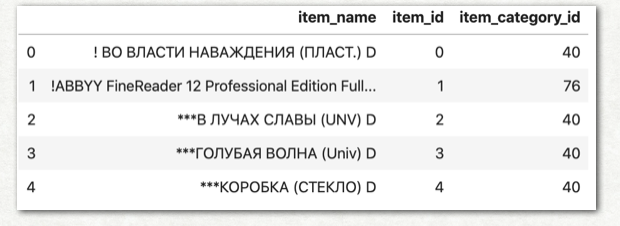
\includegraphics{test.png}
% \end{figure}

% \subsection{Tables}
% \lipsum[12]
% See awesome Table~\ref{tab:table}.

% \begin{table}
% 	\caption{Sample table title}
% 	\centering
% 	\begin{tabular}{lll}
% 		\toprule
% 		\multicolumn{2}{c}{Part}                   \\
% 		\cmidrule(r){1-2}
% 		Name     & Description     & Size ($\mu$m) \\
% 		\midrule
% 		Dendrite & Input terminal  & $\sim$100     \\
% 		Axon     & Output terminal & $\sim$10      \\
% 		Soma     & Cell body       & up to $10^6$  \\
% 		\bottomrule
% 	\end{tabular}
% 	\label{tab:table}
% \end{table}



\end{document}
